% !TEX encoding = UTF-8 Unicode
\documentclass[aodsor,preprint]{imsart}
\usepackage{amsthm,amsmath,amssymb}
\usepackage{graphicx}
\usepackage[authoryear,round]{natbib}
\usepackage[colorlinks,citecolor=blue,urlcolor=blue]{hyperref}
\usepackage[utf8]{inputenc}
\usepackage{amsmath}
\usepackage{movie15}
%\usepackage{ngerman}


% settings
%\pubyear{2005}
%\volume{0}
%\issue{0}
%\firstpage{1}
%\lastpage{8}
%\arxiv{arXiv:0000.0000}


\numberwithin{equation}{section}
\theoremstyle{plain}
\newtheorem{thm}{Theorem}[section]
\newtheorem{lemma}[thm]{Lemma}
\newtheorem{corollary}[thm]{Corollary}
\newtheorem{remark}[thm]{Remark}
\newtheorem*{remark*}{Remark}

% customize math operators
\newcommand{\E}{{\mathbb E}}
% from https://tex.stackexchange.com/questions/2705/typesetting-column-vector
\newcount\colveccount
\newcommand*\colvec[1]{
        \global\colveccount#1
        \begin{pmatrix}
        \colvecnext
}
\def\colvecnext#1{
        #1
        \global\advance\colveccount-1
        \ifnum\colveccount>0
                \\
                \expandafter\colvecnext
        \else
                \end{pmatrix}
        \fi
}


\begin{document}

\begin{frontmatter}
\title{Gradient descent based optimization algorithms}
\runtitle{Gradient descent based optimization algorithms}

\begin{aug}
\author{\fnms{a} \snm{nonymous}\ead[label=e1]{a01329095@unet.univie.ac.at}}



\runauthor{anonymous}

\affiliation{University of Vienna}

\end{aug}

\begin{abstract}
Gradient descent is an important technique to iteratively optimize a function. It is very popular thanks to the importance of neural networks, but can be used in other contexts as well. The key idea is to calculate the gradient of a function at the current position and update it using some stepsize (called learning rate in machine learning). There are a lot of gradient descent based optimization algorithms, some of them will be explored in this paper. The aim is to compare them graphically and analytically with some simulations.
\end{abstract}


\end{frontmatter}

\section{Introduction}
To perform gradient descent we calculate the gradient of the function we want to optimize. In this paper, we only consider the problem of minimizing a function $f : \mathbb{R}^d \mapsto \mathbb{R}$, parameterized by $\theta \in \mathbb{R}^d$, that is

\begin{equation} \label{eq:objFunction}
\min_{\theta} f(\theta).
\end{equation}

To obtain the minimum, we start at some random position and update this position by going some step size $\eta$ (sometimes called learning rate) in the negative direction of the gradient. This is done because the gradient points to direction of the steepest ascent and the negative gradient to the steepest descent. We iteratively should get closer to a (local) minimum, until we converge to it. The step size $\eta$ is a hyperparameter which needs to be chosen wisely, because if it is too big, the function might not converge, whereas if it is too small the function is more likely to get stuck and it takes a long time until convergence. Another important role is assigned to the starting point, since some unlucky choice might cause getting stuck at a local minimum. The closer we get to the optimum, the smaller gets the gradient and the smaller are the steps, as we can see in Figure \ref{fig:gdex1}. Our objective function to iteratively update our position (later on called parameters) is given by:
\begin{equation} \label{eq:gd}
\theta^{(t)} = \theta^{(t-1)} + \eta \nabla f(\theta^{(t-1)}),
\end{equation}

\begin{equation}
\nabla f(\theta) = \begin{pmatrix}
\frac{\partial f(\theta)_{1}}{\partial \theta_{1}} \\
\frac{\partial f(\theta)_{2}}{\partial \theta_{2}} \\
\;\;\vdots \notag \\
\frac{\partial f(\theta)_{n}}{\partial \theta_{n}} \\
\end{pmatrix}.
\label{eq:gradient}
\end{equation}

$\theta^{(t)}$ and $\theta^{(t-1)}$ are some vectors from some vector space $\mathbb{R}^d$, also called parameters later on. The $t$ stands for the number of performed iterations of the algorithm. The optimization process doesn't always converge to the optimal value, because we can get stuck in a local optimum as mentioned before. But there are conditions for our function which guarantee convergence to the global minimum, as described by \cite{shalev} in Chapter 14, which are: 

\begin{center}
\begin{itemize}
\item convexity,
\item differentiability,
\item lipschitz continuity.
\end{itemize}
\end{center}

In theory gradient descent gives a fast path to the minimum of a function. In practice we don't have all these conditions and the function is unknown most of the times, we only estimate it with some sampled data. This can help escaping a local optimum, since the function estimated from some samples will be noisy.

\begin{figure}[htb]
\centering
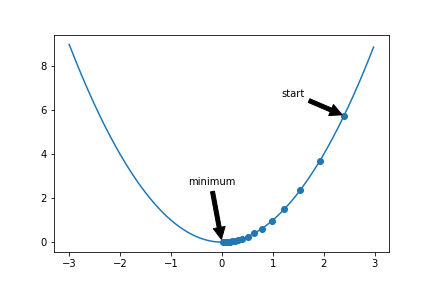
\includegraphics[width=\textwidth]{images/gd_ex1.png}
\caption{Example of $f(x) = x^2$ converging to it's minimum}
\label{fig:gdex1}
\end{figure}


\section{Types of gradient descent}
There are three variants of gradient descent, which will be briefly discussed in this section. It depends on how much data we have and how much time we want to spend calculating one update to our position. We choose different variants of gradient descent for different tasks. Since they are heavily used for machine learning tasks, we often find ourselves minimizing some cost function $f(\theta)$, with some sampled data. This means we try to find the minimum of a function we don't know, which gets modelled by a neural net. Some more context how such cost function (\ref{eq:objFunction}), in a machine learning problem looks like shall be given. In the machine learning domain, we are given some dataset with $N$ data points and sum over the losses for each sample, $f_{n}$ is the loss for the $n^{th}$ sample (\cite{Deisenroth2020}). An example for $f_{n}$ would be the negative log-likelihood

\begin{equation} \label{eq:costFunction}
f(\theta) = \sum_{n=1}^{N} f_{n}(\theta).
\end{equation}


\subsection{Stochastic gradient descent - SGD}
SGD is a variant, which takes one random sample from our dataset and updates our parameters (called $\theta$ in \ref{eq:gd}). SGD is very fast when computing the gradient, because we use only one sample. On the other hand, as described before, it makes our function very noisy and it might take more time until the function converges (\ref{fig:contour}), but it can prevent getting stuck in some local minimum (if the function is irregular and not convex). The stochasticity comes from the fact that we estimate the gradient and the function from a single sample. We introduce some randomness to the process of finding an optimum. With SGD it is harder to get close to the exact optimum, because it isn't very smooth, so when getting close we might jump around the minimum. To counteract this dilemma, one might think of the simple solution of decreasing the learning rate (step size) over time. This is actually done often to get to a better point of convergence.


\subsection{Batch gradient descent}
Batch gradient descent is often called vanilla gradient descent and uses all of our data to calculate the gradient of our cost function $f(\theta)$ from Equation \ref{eq:costFunction}. With the help of the gradient, we update our parameters with some step-size $\eta$ iteratively, until we reach some sort of convergence. For example, if the parameters haven't changed much over the last few iterations. When comparing with SGD, batch gradient descent is computationally more expensive and thus takes more time till convergence. The speed of our algorithm is also dependent on the size of our training data, since we compute the gradient over all of our data. Although it won't get faster with more data, it scales well with the number of features of our data (which is equal to n in Formula \ref{eq:gradient}). The path we take till convergence is also more stable, than when using SGD.

\begin{figure}[htb]
\centering
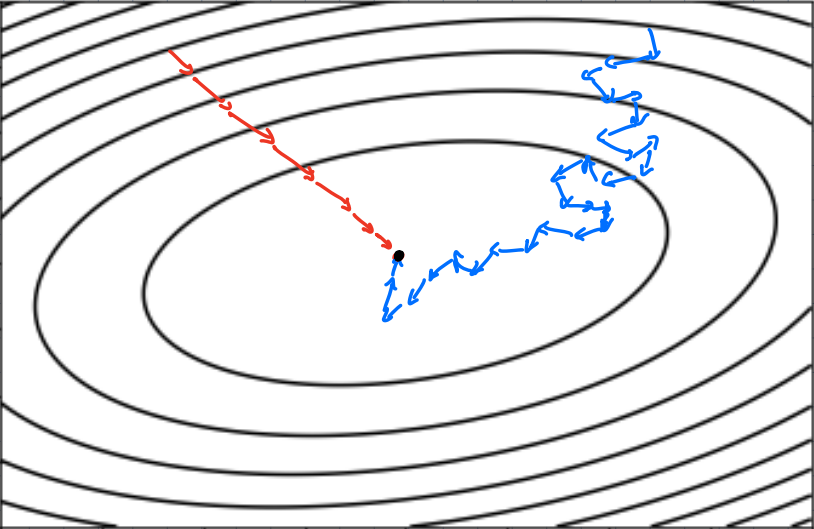
\includegraphics[scale=0.3]{images/contour.png}
\caption{contourplot of a function where the red path comes from batch gradient descent and blue from SGD}
\label{fig:contour}
\end{figure}

\subsection{Mini-batch gradient descent}
This method could be described as a mix of both variants described before. For mini-batch gradient descent we take a portion of our data (mini-batch) and perform one update to the parameters. The path till convergence wouldn't be as extreme as for SGD, but not as smooth as for the batch variant like in Figure \ref{fig:contour}. It takes the advantages from both SGD and batch gradient descent, but without their disadvantages. In most of the algorithms the parameters get updated by using mini-batches.

\section{Gradient descent based optimization algorithms}
In this section we would like to explore some optimization algorithms, which are based on gradient descent and give some intuition on how they work. There are a lot more than which will be presented, the focus will be on the most popular ones at the time of writing this paper.

\subsection{Momentum based GD}
We can imagine the idea behind this algorithm best if we think of a ball rolling down some hill. The ball starts slowly but quickly picks up momentum and accelerates until it reaches the valley, where it will slow down and eventually stop as described by \cite{geron2019hands}. Even if due to momentum, the valley will be exceeded, eventually it will be reached after some oscillation. The idea is originally proposed by \cite{polyak}.\\
Naturally the closer we get to some minimum, the smaller become the steps, that's why momentum can be quite handy to escape local minima. To get some momentum in our iterative algorithm, we not only need to consider the current gradient, but also past gradients. Mathematically we make this work by calculating some momentum vector $v$, which is updated by the gradient each iteration, and this vector then updates our parameters. The formula for momentum based gradient descent is given by:

\begin{equation} \label{eq:mgd1}
v = \beta v - \eta \nabla f(\theta),
\end{equation}

\begin{equation} \label{eq:mgd2}
\theta = \theta + v.
\end{equation}

In \ref{eq:mgd1} $\beta$ is a hyperparameter called momentum, which controls how much we depend our update $v$ on past gradients. The value of $\beta$ is between 0 and 1 and a typical default value, for example in a library like tensorflow is 0.9.

\subsection{Adagrad}\label{adagrad}
When using gradient descent, we go in the direction of the steepest slope, this means we don't directly go in the direction of the optimum. This is what adagrad, which stands for adaptive gradient wants to address. With this method, we want to correct our path, so we end up sooner at the optimum. To make this work as described by \cite{Aggarwal18}, we need to keep track of the aggregated squared magnitude of the partial derivative with respect to each parameter over the course of the algorithm. The square-root of this value is proportional to the root-mean-square slope for that parameter.
\begin{equation} \label{eq:adagrad1}
v_{i} = v_{i} + \left(\frac{\partial f(\theta)}{\partial \theta_{i}}\right)^2.
\end{equation}

\begin{equation} \label{eq:adagrad2}
\theta_{i} = \theta_{i} - \frac{\eta}{\sqrt{v_{i}}} \left(\frac{\partial f(\theta)}{\partial \theta_{i}} \right).
\end{equation}

In Equation \ref{eq:adagrad1} we keep track of the aggregated squared magnitude as mentioned before and in Equation \ref{eq:adagrad2} we update our parameters like in gradient descent scaled by $\sqrt{v_{i}}$. Note that in this section all the formulas are element-wise, before they were vector-wise. \\
As we can see in \ref{eq:adagrad1}, $v_{i}$ gets bigger and bigger and it's square root scales the learning rate down. This means, if the gradient is steep, the learning rate decays very quickly. This can become a problem for reaching the minimum, since at some point the updates will become so small that they won't change our parameters. In the next methods this problem will be fixed, by using averaging.

\subsection{RProp}
Resilient propagation is an optimization algorithm, which uses the signs of the gradient to compute the updates. It gets mentioned in this paper, because it is necessary to understand why RMSprop was introduced by Geoff Hinton. As described by \cite{RiedmillerM1993Adam} RProp performs a direct adaptation of the parameters (sometimes called weights) step based on local gradient information. The adaption is not blurred by gradient behaviour whatsoever. To make this work, we keep track of a separate learning rate $\eta_{i}$ for each dimension to update the parameter $\theta_{i}$. We need to initialize $\eta$ for the first and second iteration. The adaption rule works as follows: Every time the the partial derivative of a parameter $\theta_{i}$ changes sign, this indicates that the last update was too big and the algorithm has jumped over a local minimum, the step size $\eta_{i}$ gets decreased. In Equation \ref{eq:rprop2} we can see this behaviour, because $0<\beta<1<\alpha$ and this means that if the partial derivatives have a different sign, we multiply with $\beta$ which is less than one.

\begin{equation} \label{eq:rprop1}
\theta_{i}^{(t)} = \theta_{i}^{(t-1)} - \eta_{i}^{(t-1)}sign\left(\frac{\partial f(\theta^{(t-1)})}{\partial \theta_{i}^{(t-1)}} \right)
\end{equation}


\begin{align} \label{eq:rprop2}
\eta_{i}^{(t)} = \left\{ 
	\begin{array}{ll}
		\min{(\eta_{i}^{(t-1)}\alpha, \eta_{min})},& if \frac{\partial f(\theta^{(t)})}{\partial \theta_{i}^{(t)}} * \frac{\partial f(\theta^{(t-1)})}{\partial \theta_{i}^{(t-1)}} > 0\\
		\max{(\eta_{i}^{(t-1)}\beta, \eta_{max})}, & if \frac{\partial f(\theta^{(t)})}{\partial \theta_{i}^{(t)}} * \frac{\partial f(\theta^{(t-1)})}{\partial \theta_{i}^{(t-1)}} < 0\\
		\eta^{(t-1)}, & otherwise
	\end{array}		
\right.
\end{align}

To make sure the learning rates won't get too big or too small we use clipping values $\eta_{min}$ and $\eta_{max}$ in \ref{eq:rprop2}. The Equations are inspired from this \href{https://florian.github.io/rprop/}{website}. It is worth to note, that we used subscript $t$ to indicate the iteration of the algorithm, especially in \ref{eq:rprop2} we need this information to determine the partial derivatives in the if condition. \\
The big advantage of RProp is that the updates get calculated individually for each parameter and, this means if one is very close and another parameter is still far off, this is no problem. 

\subsection{RMSprop}
Root Mean Square Propagation was first proposed by Geoff Hinton during the Coursera course "Neural Network for Machine Learning". There was no official paper published, but the \href{https://www.cs.toronto.edu/~tijmen/csc321/slides/lecture_slides_lec6.pdf}{slides} of the lecture, which introduce the algorithm are available and give a good overview. In lecture 6e of the slides, RMSprop is explained.

\begin{equation} \label{eq:rmsprop1}
v_{i} = \beta v_{i} + (1-\beta) \left(\frac{\partial f(\theta)}{\partial \theta_{i}}\right)^2
\end{equation}

\begin{equation} \label{eq:rmsprop2}
\theta_{i} = \theta_{i} - \frac{\eta}{\sqrt{v_{i}}} \left(\frac{\partial f(\theta)}{\partial \theta_{i}} \right)
\end{equation}

RMSprop was developed by Hinton, because RProp doesn't work well with mini-batches. For example, when we consider the situation that the partial derivative of one parameter is 0.1 on nine mini-batches and -0.9 on the tenth mini-batch (using a mini-batch size of 10), the value should stay roughly where it is. RProp would increment its value 9 times and only decrease it once by about the same value. This means the parameter grows a lot, RProp has scaling issues when used together with mini-batch GD. RMSprop also addresses the problems of adaptive methods, like adagrad which where described at the end of \ref{adagrad}. \\
The problem that varying gradients can cause in RProp get mitigated in RMSprop, because we use a moving average of the squared gradient. The root of this moving average is then used to scale the gradient update accordingly as we can see in Equation \ref{eq:rmsprop2}. In Equation \ref{eq:rmsprop1} we use a parameter $\beta$ for the moving average which is set to 0.9 in the lecture slides.

\subsection{Adam}
The Adaptive Moment Estimation algorithm is very popular and is another method that computes adaptive learning rates for each parameter. It is basically a combination of RMSprop and momentum. We keep track of an exponentially decaying average of past gradients (\ref{eq:adam1}) like in momentum and we also keep track of the squared average of past gradients (\ref{eq:adam2}), which we do in RMSprop. As described by \cite{adam}, some of the advantages of this algorithm are, that the magnitudes of parameter updates are invariant to rescaling the gradient, the stepsizes are bounded by the stepsize of the hyperparameter and it works for sparse gradients.

\begin{equation} \label{eq:adam1}
u = \beta_{1} u + (1-\beta_{1}) \nabla f(\theta)
\end{equation} 

\begin{equation} \label{eq:adam2}
v = \beta_{2} v + (1-\beta_{2}) \left( \nabla f(\theta)\right)^2
\end{equation}

\begin{equation} \label{eq:adam3}
\hat{u} = \frac{u}{1-\beta_{1}^t}
\end{equation} 

\begin{equation} \label{eq:adam4}
\hat{v} = \frac{v}{1-\beta_{2}^t}
\end{equation}

\begin{equation} \label{eq:adam5}
\theta = \theta - \eta \frac{\hat{u}}{\sqrt{\hat{v}} + \epsilon}
\end{equation}

In Equation \ref{eq:adam2} the square of the gradient is an element-wise operation and in \ref{eq:adam3} and \ref{eq:adam4} $\beta_{1}$ and $\beta_{2}$ are taken to the t'th power, where t is the iteration of the algorithm. A common value for the hyperparameter $\beta_{1}$ is 0.9 and 0.999 for $\beta_{2}$. The adam optimizer bias corrects $u$ and $v$, the bias corrected versions are $\hat{u}$ and $\hat{v}$, which are used to update our parameters. We need this bias correction, because at the start of the algorithm $u$ and $v$ will be initialized with zero and therefore biased towards the initialized value.
The $\epsilon$ in \ref{eq:adam5} is a smoothing term and usually some small value like $10^{-8}$ is chosen. \cite{geron2019hands} mentions that adam requires less tuning of $\eta$ than the algorithms presented before.

\section{Comparing the different algorithms}
The goal for this section is, to compare the different algorithms graphically and also empirically. For the visual method a simple program was written which tracks the paths of different algorithms on contourplots. For the empirical comparision, a simple model was defined and the performance of the different algorithms were compared, with synthetic data.

\subsection{Graphical method}
The goal for this section is to compare the discussed optimization algorithms with some plots, which show their different paths to the minimum. The implementation was done in python3 with anaconda (the code is available as .py files too) and jupyter-notebook using pyplot from matplotlib for plotting and tensorflow to calculate the gradients of the functions. The code is available at \href{https://github.com/}{github}. \\
Most of the discussed optimization algorithms are implemented and can be used to visualize them in a 2D- or 3D-contour-plot. All optimizers implement the abstract class optimizer, to give them the same structure. The abstract method apply\_gradients is implemented in each of them, which is then used to update the parameters according to the algorithm. The main class is min\_function, which is initialized with a function (needs to be a 3D-function), a starting point (start), the global minimum (global\_min), which is needed to check if the gradient descent has reached the optimium, a learning rate (learning\_rate) and a list of optimizers which we want to compare. When creating an object of min\_function the calculation heavy stuff is done during the creation, because we minimize the function for all optimizers. This is done by calling minimize for every optimizer, we initialize two parameters with the starting point and create lists to store the values at each iteration (to later plot them). Then we calculate the gradient and update the parameters by using the implemented optimizers iteratively and we stop when we are really close to the minimum. The function plot2d creates a 2D-contourplot and also plots the values, which where calculated and stored in lists before. Plot3d does exactly the same just in 3D. In the 3 dimensional case we can even rotate our function and have a look from different directions. We can even create a gif of the 2D-plots with the function create\_gif, to see the different paths evolving for all methods. It is recommended to run this part using python together with the .py files.

\begin{figure}[htb]
\centering
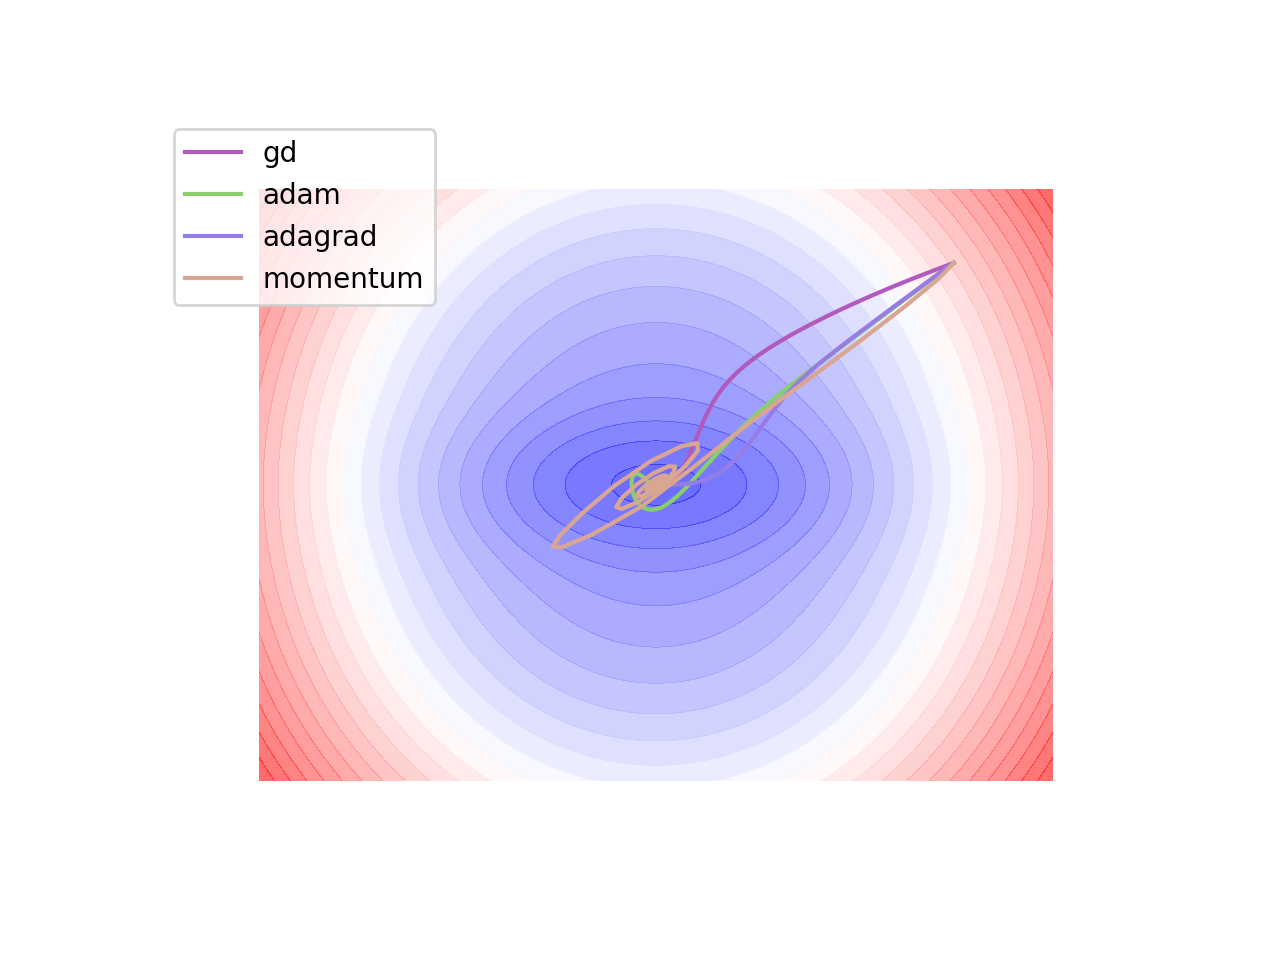
\includegraphics[scale=0.7]{images/compare1.png}
\caption{2D-contpourplot of a bowl shaped function displaying the paths of different algorithms}
\label{fig:contour1}
\end{figure}

\begin{figure}[htb]
\centering
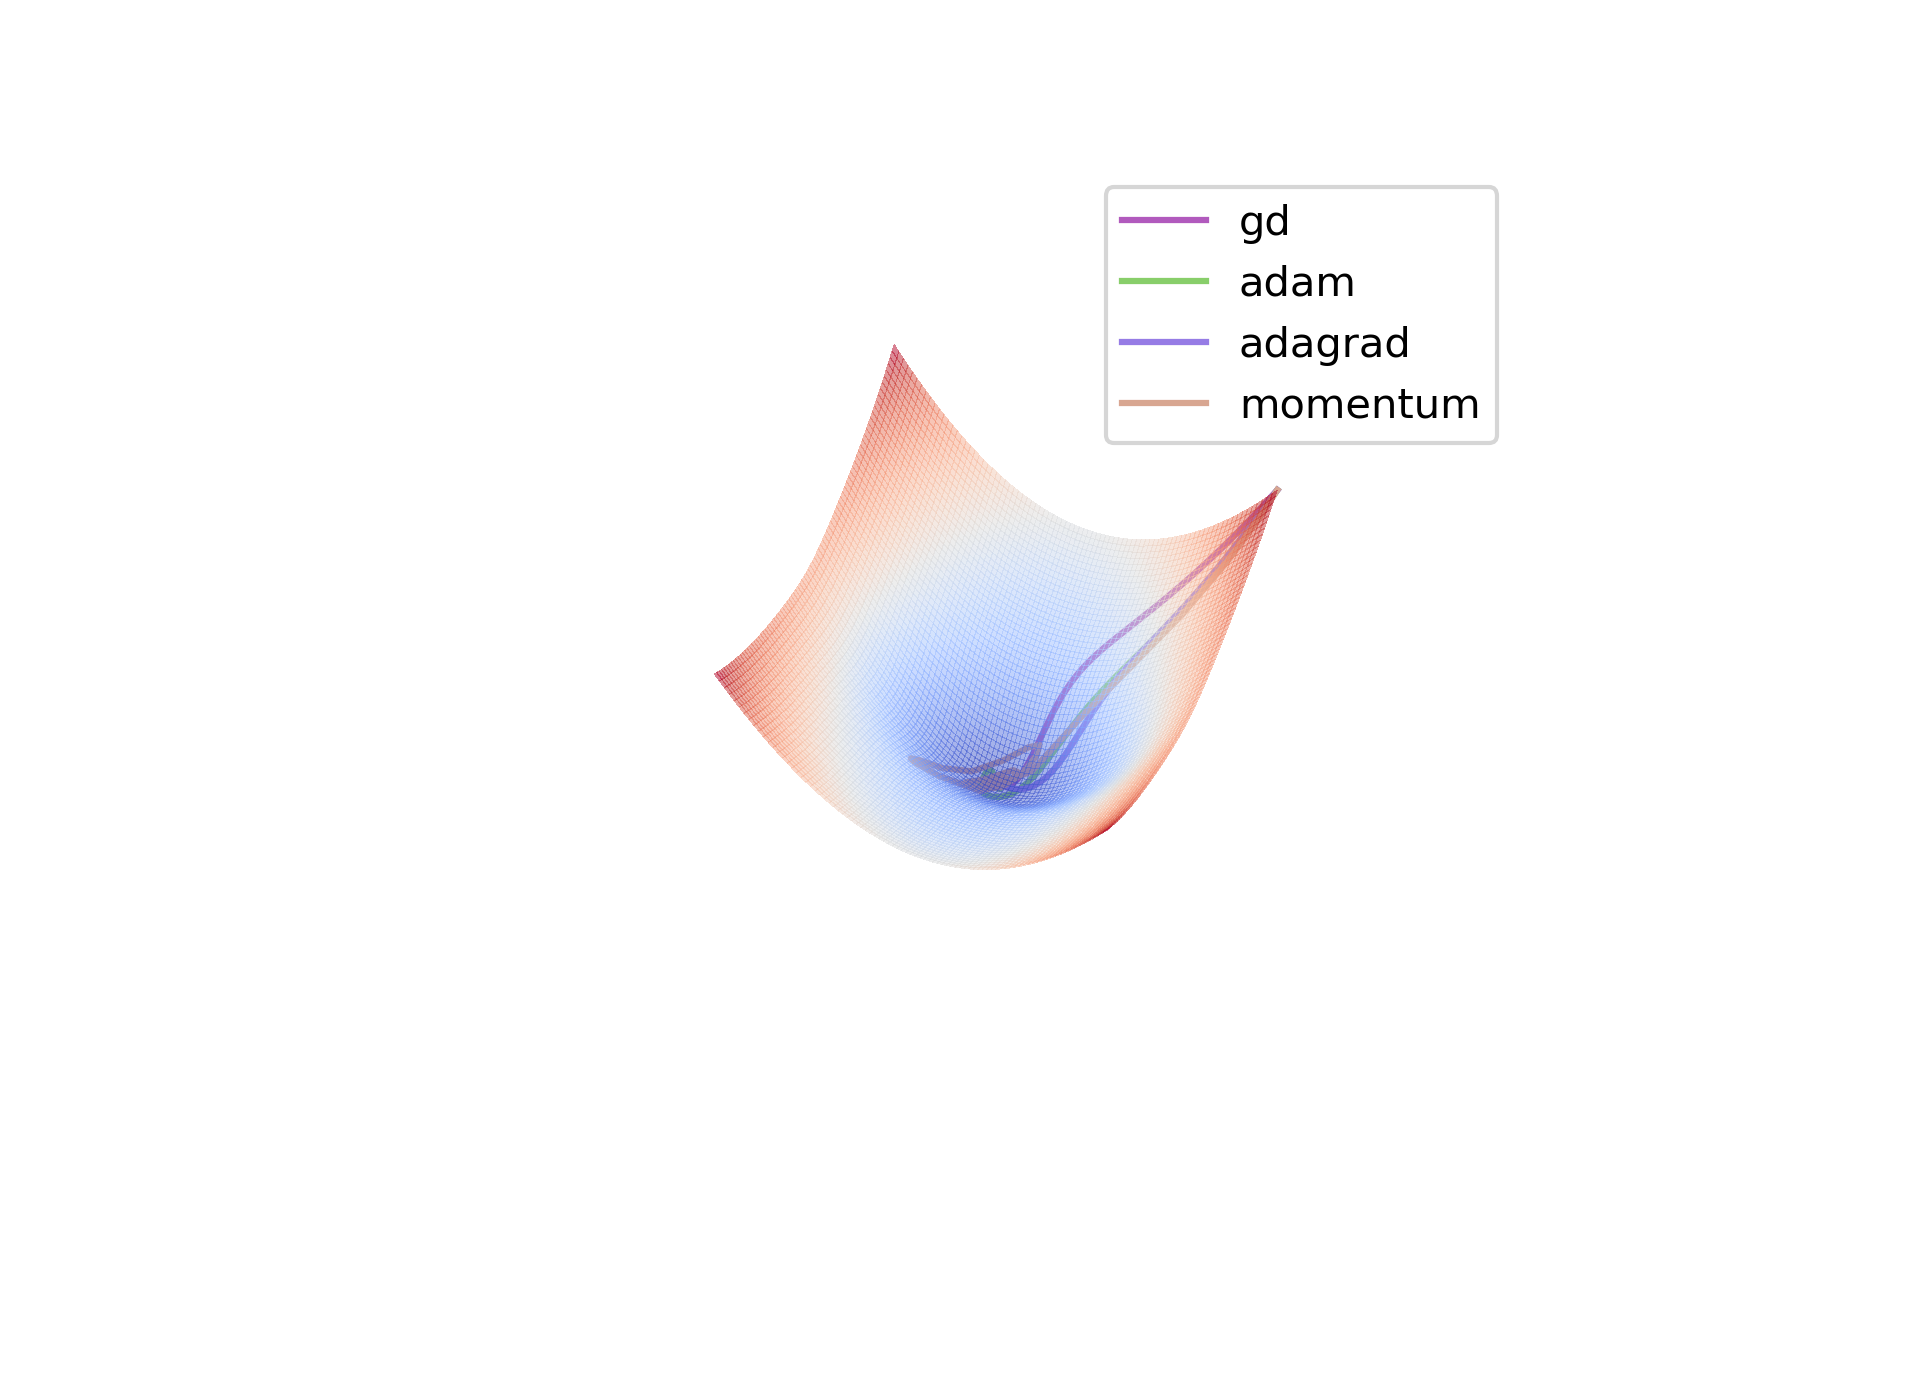
\includegraphics[scale=0.7]{images/compare2.png}
\caption{3D-contpourplot of a bowl shaped function displaying the paths of different algorithms}
\label{fig:contour2}
\end{figure}

\subsection{Simulations}
For the empirical comparison of the different algorithms, which were introduced before, a simple model is defined to measure their performance:

\begin{equation}
y = X^{t} \theta + \epsilon,
\end{equation}

\begin{equation}
\epsilon \sim \mathcal{N}(0, \sigma^{2}\mathit{I}_n), \quad \sigma^{2} = 0.1,
\label{eq:model}
\end{equation}

\begin{equation}
X \sim \exp (1).
\end{equation}

X is a 5000x3 matrix sampled from an exponential distribution as specified in \ref{eq:model}. The model has no intercept, this means the bias in the simple regression model should be zero. The parameter $\theta$ of the underlying model is 
$\begin{pmatrix} 2 & 1 & 4 \end{pmatrix}^{t}$ and $\epsilon$ is used as some sort of noise. The model is initialized randomly, this means the initial $\theta$ is a random value and then the optimization algorithms are iteratively used to find the optimal value for $\theta$. In a simple simulation, for each algorithm a model was trained for 20 times for 50 epochs and then the weights (values for $\theta$) were averaged for the 20 simulations for each epoch (a epoch is one run over the entire training set). As a loss function the mean squared error was used. There was one simulation run for a learning rate of 0.01 which is summarised in \ref{fig:simulation1}. We can see the true values for the parameters marked by a dotted line, which is black. When choosing a learning rate of 0.01, we can observe that RMSProp performs the best and is closest to the true values of the parameters. Surprisingly sgd performs very well and isn't far off as well. In the summary statistics for the adam optimizer, we can see in the row for the minimum, that there are some outliers. When looking through all values it was clear, that the algorithm got stuck in a local minimum and the values of the weights didn't change at all. This can be prevented, by either adapting the learning rate or using a different initialization method of the weights. Since there is one iteration of the 20 simulation runs, the mean is way off when comparing to the other algorithms. One interesting observation is, all algorithms in \ref{fig:simulation1} approximately converge to the true bias (which is zero), but with adagrad the bias gets bigger and bigger. \\
The same simulations were run with a learning rate of 0.1 and are summarised in Figure \ref{fig:simulation2}. In this graphic we can observe, that adam and adagrad are closest to the true values after 50 observations, although adagrad definitely takes longer. When looking at RMSProp, we can see that a bigger learning rate makes this algorithm unstable and not as smooth as the rest. With sgd it seems like it doesn't change at all, but we have to keep in mind, that the values of the parameters get saved only at the end of an epoch. This means a change from the initialization to the the end of the first epoch doesn't show up in the plot. It has to be mentioned, that most of the times the true values are found, but if an algorithm gets stuck in the beginning at some value which is far off, the mean over all 20 simulations is impacted heavily by that. When looking at the collected data (which is not shown here since it is a hige matrix), it could be seen that most of the times algorithms had a good performance, but a few times they got stuck and the values didn't change any more. The same summary statistics are provided exemplary for adam in \ref{fig:sumstat2} as before.\\
The code for the simulations is also done using python and tensorflow and can be found in the jupyter notebook.

\begin{figure}[htb]
\centering
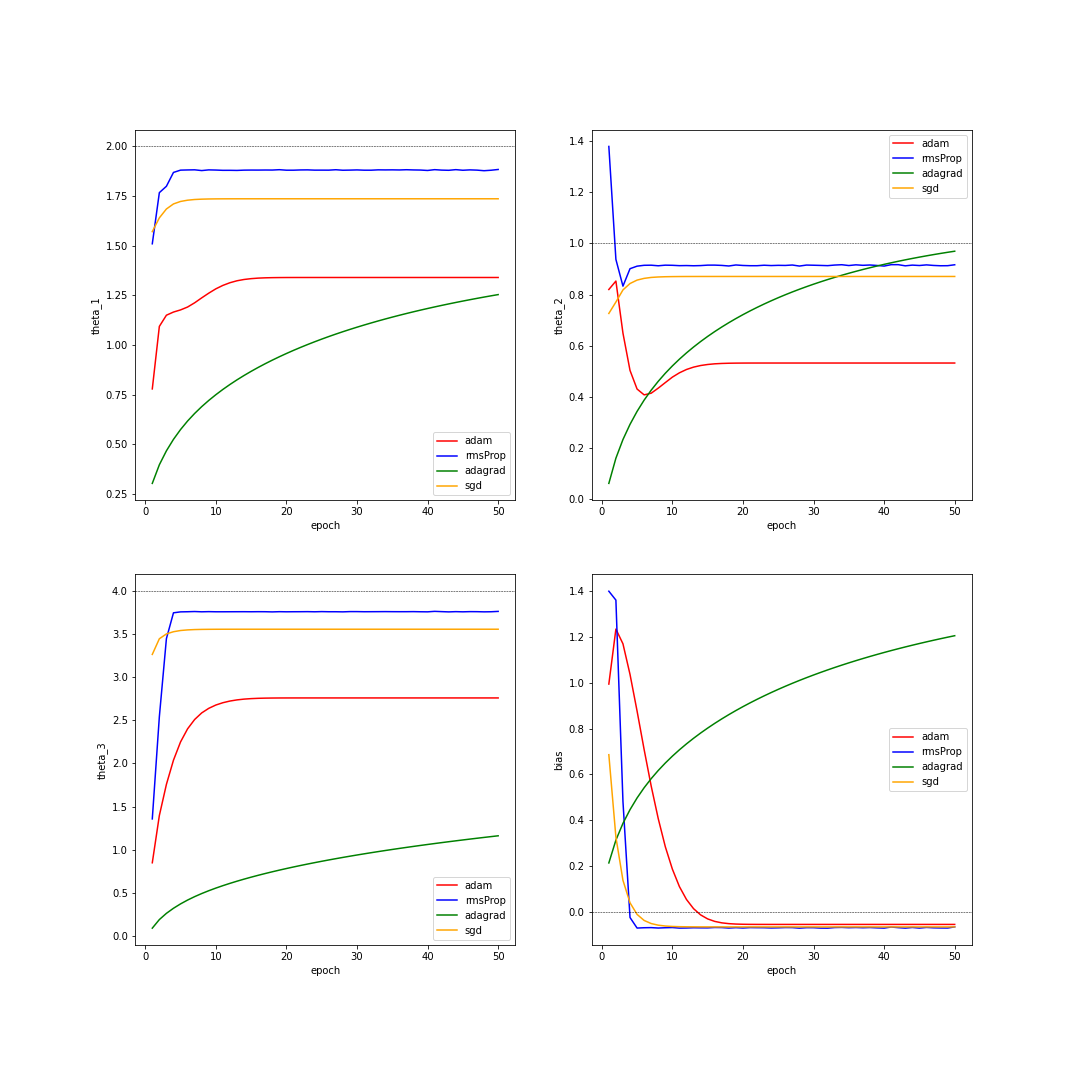
\includegraphics[scale=	0.37]{images/comparison1.png}
\caption{Comparision of the different gradient based optimization algorithms, with learning rate 0.01}
\label{fig:simulation1}
\end{figure}

\begin{figure}
\centering
\begin{tabular}{l|llll}
 &  $\theta_{1}$ &  $\theta_{2}$ &  $\theta_{3}$ & bias \\ \hline
mean  &  1.300961 & 0.532996 & 2.627780 & 0.114192\\
std   &  1.160185 & 0.849872 & 2.127005 & 0.076019\\
min   & -1.161238 & -1.210704 & -1.184551 & 0.000000\\
25\%   & 1.363470 &  0.630324 & 2.674388 & 0.020478\\
50\%   & 1.930871 &  0.985981 & 3.797112 & 0.149574\\
75\%   & 1.958200 &  1.014009 & 3.823697 & 0.171807\\
max   & 1.986382 &  1.028341 & 3.910801 & 0.186259\\
\end{tabular}
\caption{Summary statistics for simulations with adam with a learning rate of 0.01.}
\label{fig:sumstat1}
\end{figure}

\begin{figure}[htb]
\centering
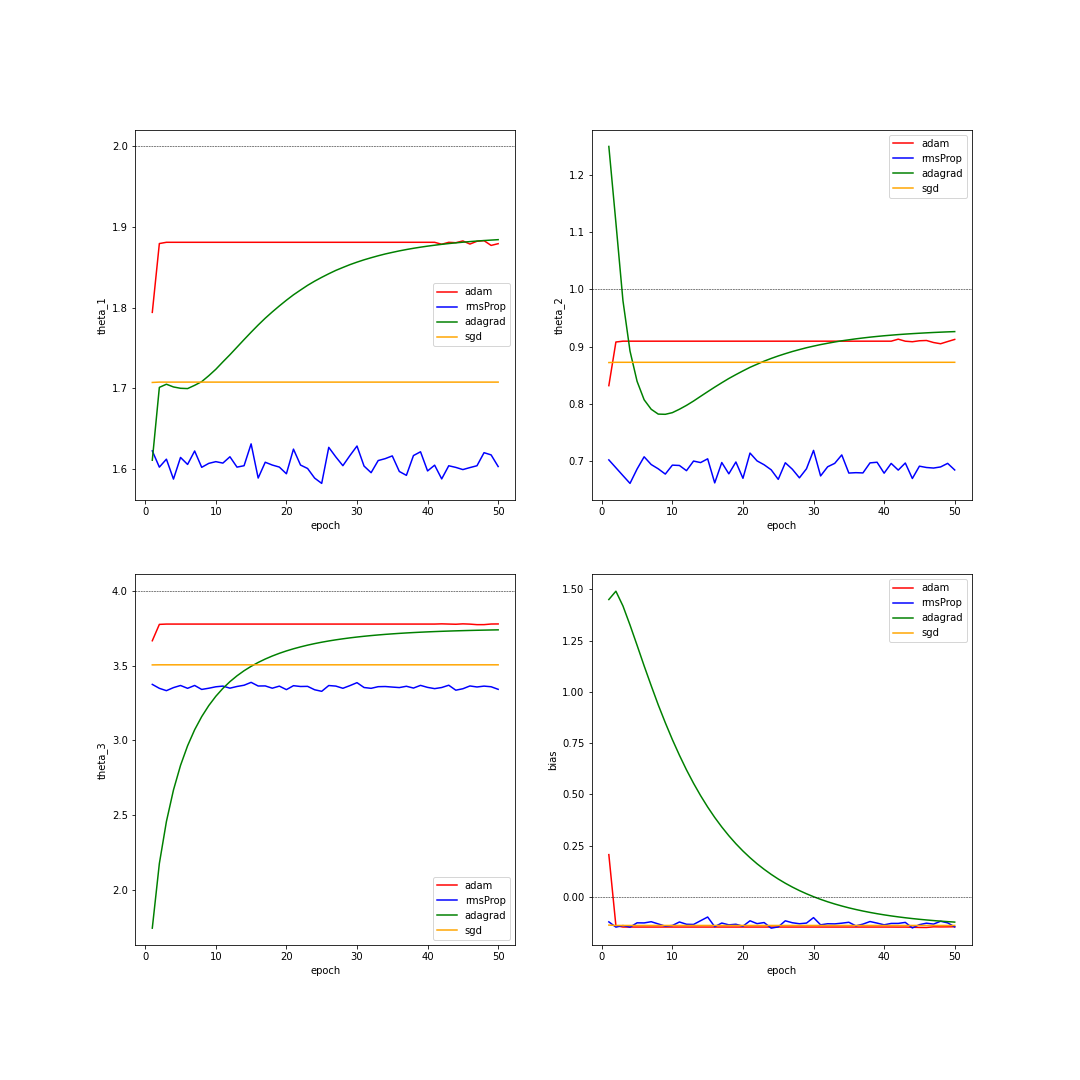
\includegraphics[scale=	0.37]{images/comparison2.png}
\caption{Comparision of the different gradient based optimization algorithms, with learning rate 0.1}
\label{fig:simulation2}
\end{figure}

\begin{figure}
\centering
\begin{tabular}{l|llll}
 &  $\theta_{1}$ &  $\theta_{2}$ &  $\theta_{3}$ & bias \\ \hline
mean  &  1.879290 & 0.907825 & 3.777316 & -0.139256\\
std   &  0.530963 & 0.404750 & 0.984651 & 0.032921\\
min   & -0.376518 & -0.811759 & -0.405998 & -0.153006\\
25\%   & 1.997565 &  0.997612 & 3.996688 & -0.148435\\
50\%   & 1.998073 &  0.998246 & 3.997715 & -0.146279\\
75\%   & 1.998422 &  0.998563 & 3.998211 & -0.144599\\
max   & 1.999311 &  1.001173 & 4.000235 & 0.000000\\
\end{tabular}
\caption{Summary statistics for simulations with adam with a learning rate of 0.1.}
\label{fig:sumstat2}
\end{figure}

\section{Conclusion}
The main goal of this work is to explain different gradient descent based optimization algorithms and develop a program which lets someone compare them graphically. There is still room for improvement in the provided implementation, further algorithms can be added easily. One disadvantage is that the colouring of the paths is random, so sometimes we can end up with pretty similar colors. When looking at the data of the simulations, it is clear that random initialization sometimes is responsible for getting stuck in a local minimum. If one run gets stuck at values which are far from the true values, than the mean is impacted heavily since it is not resistant to outliers. Some further analysis on when the different algorithms get stuck and how often they get stuck could be done in the future.


\section{Acknowledgements}
I would like to thank the reviewer, which helped a lot to improve this paper.

\bibliographystyle{imsart-nameyear}
\bibliography{lit}{}

\end{document}